%%%%%%%%%%%%%%%%%%%%%%%%%%%%%%%%%%%%%%%%%
% University/School Laboratory Report
% LaTeX Template
% Version 3.1 (25/3/14)
%
% This template has been downloaded from:
% http://www.LaTeXTemplates.com
%
% Original author:
% Linux and Unix Users Group at Virginia Tech Wiki
% (https://vtluug.org/wiki/Example_LaTeX_chem_lab_report)
%
% License:
% CC BY-NC-SA 3.0 (http://creativecommons.org/licenses/by-nc-sa/3.0/)
%
%%%%%%%%%%%%%%%%%%%%%%%%%%%%%%%%%%%%%%%%%

\documentclass{article}

%\usepackage[version=3]{mhchem} % Package fo  r chemical equation typesetting
%\usepackage{siunitx} % Provides the \SI{}{} and \si{} command for typesetting SI units
\usepackage{graphicx} % Required for the inclusion of images
\usepackage{natbib} % Required to change bibliography style to APA
\usepackage{amsmath} % Required for some math elements
\usepackage{listings}
\usepackage{graphicx}
\usepackage{hyperref}
\usepackage{cleveref}
\usepackage{tikz}
\usepackage{subfigure}
\usepackage{caption}
\usepackage{float}
\usepackage{siunitx}

\lstset{basicstyle=\ttfamily, breaklines=true}
\setlength\parindent{2pt} % Removes all indentation from paragraphs
\linespread{1.5}
%\renewcommand{\labelenumi}{\alph{enumi}.} % Make numbering in the enumerate environment by letter rather than number (e.g. section 6)

%\usepackage{times} % Uncomment to use the Times New Roman font


%----------------------------------------------------------------------------------------
%	DOCUMENT INFORMATION
%----------------------------------------------------------------------------------------

\title{Design of Foscam Webcam Firmware\\ UML for Embedded Systems} % Title

\author{Simone \textsc{Rossi}} % Author name


\date{\today} % Date for the report

\begin{document}

\maketitle % Insert the title, author and date

\begin{center}
\begin{tabular}{l r}
Date Performed: & \today \\ % Date the experiment was performed
Partners: & Simone Rossi \\ % Partner names
%& Mary Smith \\
%Instructor: & Professor Smith % Instructor/supervisor
\end{tabular}
\end{center}

% If you wish to include an abstract, uncomment the lines below
% \begin{abstract}
% Abstract text
% \end{abstract}

%----------------------------------------------------------------------------------------
%	SECTION 1
%----------------------------------------------------------------------------------------

\section{Assumptions}
\begin{itemize}
\item \textbf{LightSensor\_value\_rate}: the light sensor provides a valid data
once per second
\item \textbf{Camera\_frame\_rate}: the camera provides a valid frame every 1/25
sec (40 ms)
\item \textbf{Request\_notification}: each incoming Ethernet request is preceeded
by a request notification
\item \textbf{QR\_configuration}:  the QR code is the serial number of the camera.
During configuration, the serial read by the smartphone is compared with the
internal serial number. If equal, then the communication is configured
\item \textbf{Recording\_video}: If the camera has been configured, it always
records video and checks for motion objects.
\end{itemize}

\newpage

\section{Block Diagram}
In my design of the Foscam Firmware, the main controller is divided into five
different submodules, each of them specialized for one particular task.
\\
To be more realistic, the design includes also the definition of three custom
types: Email, Image and Video.
\begin{figure}[!h]
  \centering
  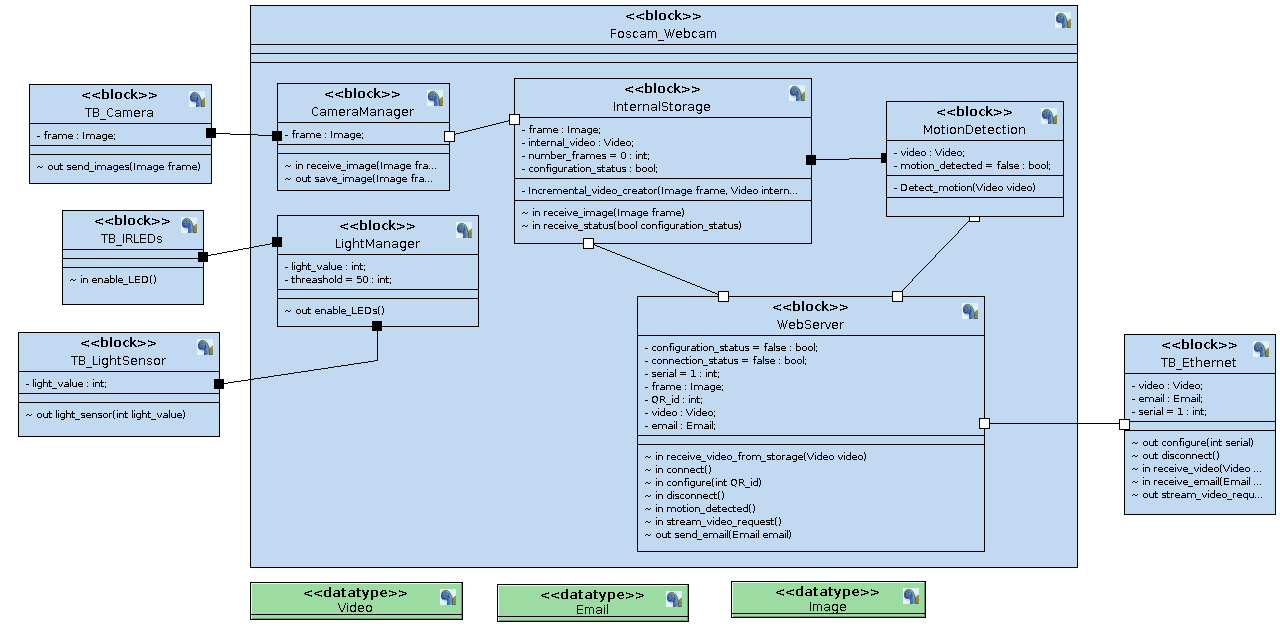
\includegraphics[width=\textwidth]{./Foscam00.png}
  \caption{Main blocks with their testbench modules}
\end{figure}

\subsection{Light Manager}
\label{sec:Light Manager}

\begin{minipage}{\linewidth}
  \centering
  \begin{minipage}{0.6\linewidth}
    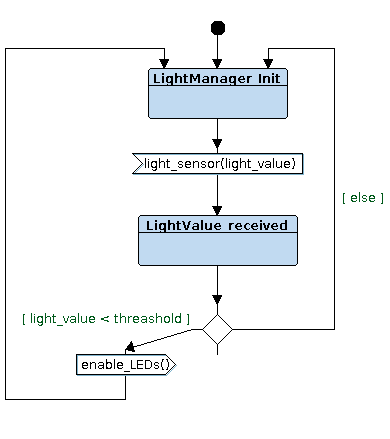
\includegraphics[width = \textwidth]{Foscam06.png}
  \end{minipage}
  \begin{minipage}{0.35\linewidth}
    The \texttt{Light Manager} simply waits for a new value from the light sensor
    and if it is higher than a given threashold, it drives the signal \texttt{enable\_LED},
    which will be eventually received by the IR LEDs module.
  \end{minipage}
\end{minipage}

\subsection{Camera Manager}
\label{sec:Camera Manager}

\begin{minipage}{\linewidth}
  \centering
  \begin{minipage}{0.6\linewidth}
    \centering
    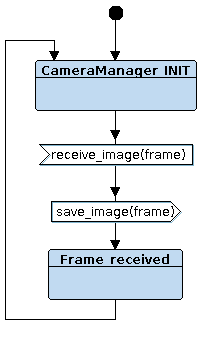
\includegraphics[width = 0.5\textwidth]{Foscam08.png}
  \end{minipage}
  \begin{minipage}{0.35\linewidth}
    The \texttt{Camera Manager} is in charge of receiving the video frame by frame
    and create a stream for the \texttt{Internal Storage}.
  \end{minipage}
\end{minipage}

\subsection{Internal Storage}
\label{sec:Internal Storage}

\begin{minipage}{\linewidth}
  \centering
  \begin{minipage}{0.60\linewidth}
    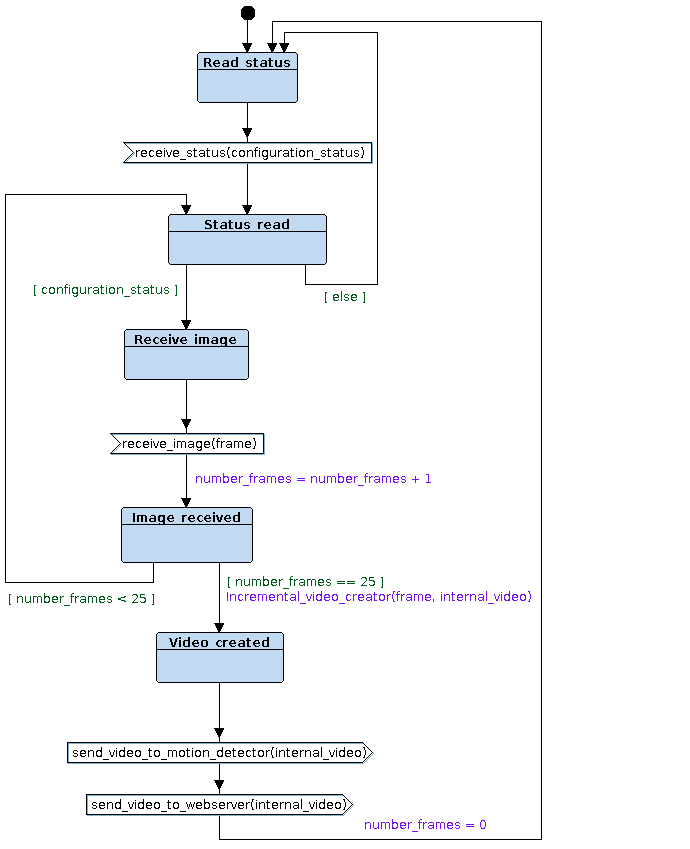
\includegraphics[width = \textwidth]{Foscam07.png}
  \end{minipage}
  \begin{minipage}{0.35\linewidth}
    If the camera has been configured, the \texttt{Internal Storage} will start
    receiving images and after 25 frames (e.g. 1 second) the video is created
    and stored. As soon as a video is created, it will be send both to the
    \texttt{Ethernet Interface} and to the embedded \texttt{Motion Detection}
    engine.
  \end{minipage}
\end{minipage}

\subsection{Motion Detector}
\label{sec:Motion Detector}

\begin{minipage}{\linewidth}
  \centering
  \begin{minipage}{0.6\linewidth}
    \centering
    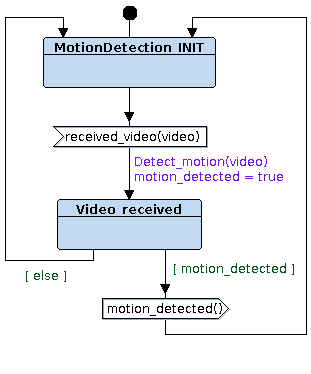
\includegraphics[width = 0.8\textwidth]{Foscam10.png}
  \end{minipage}
  \begin{minipage}{0.35\linewidth}
    The motion detection engine will analyse a one second video to eventually
    identify some moving objects. If so, the WebServer will be notified and
    an alarm will be triggered.
  \end{minipage}
\end{minipage}

\newpage
\subsection{WebServer}
\label{sec:WebServer}

\begin{figure}[h!]
  \centering
  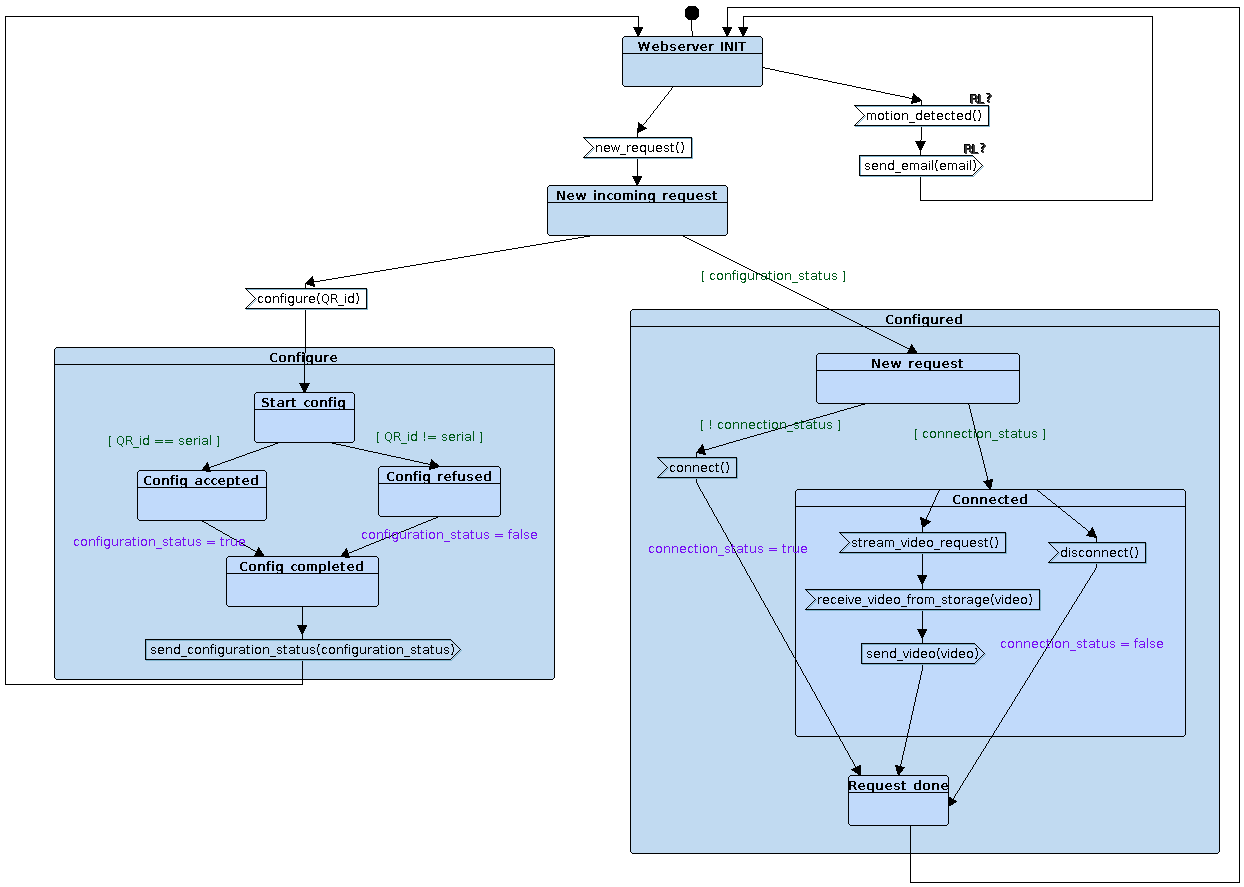
\includegraphics[width = \textwidth]{Foscam09.png}
\end{figure}

This is the most complex submodule of the firmware. This module is used for:
\begin{itemize}
  \item \textbf{Configuration} and pairing to a new smartphone/computer using
    a QR code;
  \item \textbf{Connection} and \textbf{disconnection} of a configured
    smartphone/computer;
  \item \textbf{Stream video} if required by the user;
  \item \textbf{Alarm Management} if the detection engine has triggered an
    object movement.
\end{itemize}

\section{Nominal Case Diagrams}
\label{sec:Nominal Cases Diagram}
These are some nominal case diagrams used to understant whether or not all
the subsystems work as stated in the requirements.

\subsubsection{Light Management}
\label{subs:Light Management}
\begin{figure}[h!]
  \centering
  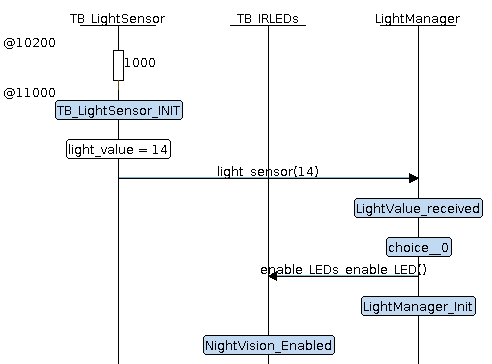
\includegraphics[width = 0.7\textwidth]{./light_sensor.png}
\end{figure}

\subsubsection{Camera Management}
\label{subs:Light Management}
\begin{figure}[h!]
  \centering
  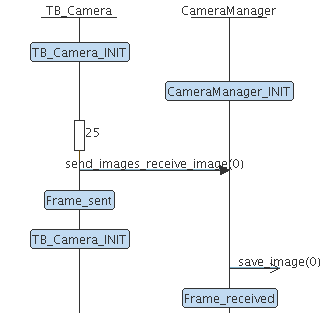
\includegraphics[width = 0.7\textwidth]{./camera_management.png}
\end{figure}
\newpage
\subsubsection{WebServer}
\label{subs:Light Management}
\begin{figure}[h!]
  \centering
  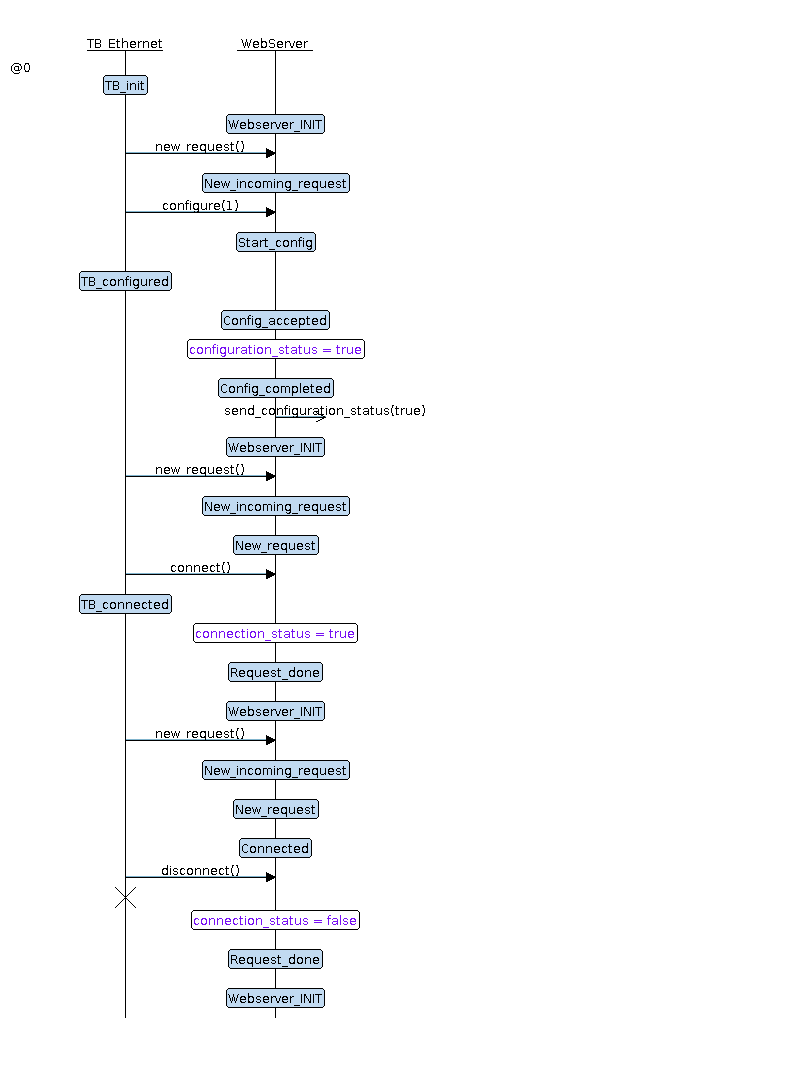
\includegraphics[width = .65\textwidth]{./disconnection_from_ethernet.png}
\end{figure}


\section{Formal Verification}
\label{sec:Formal Verification}

For the formal verification, I verified that whenever a moving object has been
detected, an email will be send. The formal proof has shown that both these states
are reachable and the liveness property is guaranteed.
\begin{figure}[!h]
  \centering
  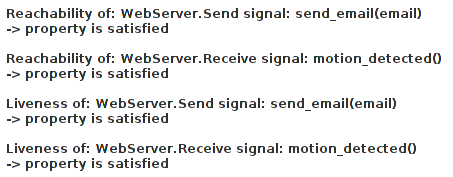
\includegraphics[width = \textwidth]{./formal_verification.png}
\end{figure}

\end{document}
